%Version 2.1 April 2023
% See section 11 of the User Manual for version history

%%\documentclass[pdflatex,sn-basic]{sn-jnl}% Basic Springer Nature Reference Style/Chemistry Reference Style
\documentclass[referee,pdflatex,sn-basic]{sn-jnl}% referee := double spacing

\usepackage{graphicx}%
\usepackage{multirow}%
\usepackage{amsmath,amssymb,amsfonts}%
\usepackage{amsthm}%
\usepackage{mathrsfs}%
\usepackage[title]{appendix}%
\usepackage{xcolor}%
\usepackage{textcomp}%
\usepackage{manyfoot}%
\usepackage{booktabs}%
\usepackage{algorithm}%
\usepackage{algorithmicx}%
\usepackage{algpseudocode}%
\usepackage{listings}%
%%%%

\usepackage[super]{nth}% for superscripts


\theoremstyle{thmstyleone}%
\newtheorem{theorem}{Theorem}%  meant for continuous numbers
\newtheorem{proposition}[theorem]{Proposition}% 

\theoremstyle{thmstyletwo}%
\newtheorem{example}{Example}%
\newtheorem{remark}{Remark}%

\theoremstyle{thmstylethree}%
\newtheorem{definition}{Definition}%

\raggedbottom
%%\unnumbered% uncomment this for unnumbered level heads

\begin{document}

\title[Article Title]{Adaptive, functional and phylogenetic insights of 114 plants based on orthologous categories 
% Protein diversity in plant proteomes: 
% Elucidating evolutionary relationships through amino acid analysis
}

%%=============================================================%%
%% Prefix	-> \pfx{Dr}
%% GivenName	-> \fnm{Joergen W.}
%% Particle	-> \spfx{van der} -> surname prefix
%% FamilyName	-> \sur{Ploeg}
%% Suffix	-> \sfx{IV}
%% NatureName	-> \tanm{Poet Laureate} -> Title after name
%% Degrees	-> \dgr{MSc, PhD}
%% \author*[1,2]{\pfx{Dr} \fnm{Joergen W.} \spfx{van der} \sur{Ploeg} \sfx{IV} \tanm{Poet Laureate} 
%%                 \dgr{MSc, PhD}}\email{iauthor@gmail.com}
%%=============================================================%%

\author*[1,2]{\fnm{Nicolás} \sur{López-Rozo}}\email{nicolaslopez@javerianacali.edu.co}

\author[3]{\fnm{Fabian} \sur{Tobar-Tosse}}

\author[1,2]{\fnm{Jorge} \sur{Finke}}

\author[1,2]{\fnm{Camilo} \sur{Rocha}}\email{camilo.rocha@javerianacali.edu.co}


\affil*[1]{\orgdiv{Department of Electronics and Computer Science}, \orgname{Pontificia Universidad Javeriana Cali}, \orgaddress{\street{Calle 18 No. 118-250}, \city{Cali}, \postcode{111021}, \state{Valle del Cauca}, \country{Colombia}}}

\affil[2]{\orgdiv{OMICAS program}, \orgname{Pontificia Universidad Javeriana Cali}, \orgaddress{\street{Calle 18 No. 118-250}, \city{Cali}, \postcode{111021}, \state{Valle del Cauca}, \country{Colombia}}}

\affil[3]{\orgdiv{Department of Health Sciences}, \orgname{Pontificia Universidad Javeriana Cali}, \orgaddress{\street{Calle 18 No. 118-250}, \city{Cali}, \postcode{111021}, \state{Valle del Cauca}, \country{Colombia}}}

%%================================%%
%% Sample for structured abstract %%
%%================================%%

\abstract{

% \textbf{Abstract}
% Proteins are essential for the functioning of cells in living 
% organisms, including plants. This study examines the protein 
% sequences of 114 plants, as well as 
% the related annotations using the concept of Eukaryotic 
% orthologous groups (KOGs). Based on the KOG category counts 
% of annotated proteins, a hierarchical classification that 
% groups similar plants is carried out, providing insights 
% into their shared evolutionary histories and adaptation 
% strategies. We also compare Gene Ontology and KOG categories 
% and find a strong correlation between the two rankings, 
% supporting the reliability of our results. These findings have 
% important implications for understanding plant speciation, 
% interactions in their environment, and responses to changing 
% conditions.

Functional annotations in plant genomes are essential 
for defining adaptive mechanisms under different stress 
conditions. In comparison to animals, plants exhibit a higher 
degree of diversification and sophistication by its non-locomotive 
capacity. However, some functional enrichments in multi-omics
approaches lack confidence due to their fuzzy phenotypic 
associations. Therefore, this study introduces new approaches 
based on biological insights. Here, an exploration of 
114 plant proteomes elucidates singularities in 
functional prioritization based on orthologous genes and their 
implications for plant adaptative properties. Results reveal 
distinct trends in the density of functional annotations 
for physiologically distant groups (Eudicots, Monocots, Algae). 
Furthermore, certain functional categories show relevance in 
the classification of plants. Lastly, the 
frequency patterns within these groups are proposed as 
insights into the distribution of functional groups for other 
organisms.


\textbf{Main Conclusion} 
This study unveils a hierarchical structure in 114 plant 
proteomes based on KOG category frequencies, resembling 
phylogenetic taxonomy for two plant clusters and showing
differentiated trends in annotation distributions for three 
groups of plants. Additionally, noticeable correlations 
between Phytozome and Gene Ontology annotations support 
reliable insights into plant speciation and adaptation 
mechanisms. 

}
\keywords{
Bioinformatics,
Functional diversity,
Hierarchical classification,
Comparative analysis,
Gene Ontology}

\maketitle

\subsection*{Abbreviations}

KOG: euKaryotic Orthologous Groups

COG: Clusters of Orthologous Genes

GO: Gene Ontology

BLASTP: Basic local alignment search tool for proteins

%%%%%%%%%%%%%%%%%%%%%%%%%%%%%%%%%%%%%%%%%%
\section{Introduction}
\label{sec:intro}
%% Why bother?
Proteins, as the building blocks of life on Earth, play a 
crucial role in cellular maintenance, replication, and defense 
across all living organisms~\citep{kaur2022}. They are involved 
in diverse cellular functions, including signal transduction, 
regulation of metabolic pathways, and responses to environmental 
stimuli~\citep{zhang2010}.

The study of proteins and their functions is a central focus in 
molecular biology and bioinformatics research. Understanding the 
biological function of proteins, also known as functional 
annotations, is essential for comprehending 
the genetics of an organism~\citep{silva2020}. Furthermore, these 
functional annotations are useful when computationally improving 
classification or correlation tasks on proteins, especially those 
involving noisy data. 

Among living 
organisms, plants hold particular significance due to their 
vital roles in photosynthesis and the establishment of various 
ecosystems. Moreover, their adaptive mechanisms consist of a 
wide range of molecular processes, many of which still remain 
unidentified. The Plantae kingdom, encompassing a vast array of 
species, exhibits unparalleled diversity in protein sequences 
that have evolved over millions of years~\citep{chaudhary2019}. 
Such diversity arises from complex gene regulation processes 
that define cell response to stimuli or plant adaptation, 
including co-transcriptional, post-transcriptional, and 
post-translational regulation~\citep{skelly2016}. In 
consequence, analyzing 
patterns and variations within plant protein sequences can 
provide invaluable insights into their evolutionary history 
and adaptations to different ecological niches, which could be 
used in current analysis methods to establish 
relationships among plant species.

When assessing adaptive mechanisms in plant cells, the 
identification of proteins or their unique attributes
involves an intricate process due to the complexity of plant 
genomes and their expression products. Although 
computational models enhance the definition of significant elements 
in plant cell biology, this process could potentially lead to an 
extrapolation of overrepresented information from databases, rather 
than capturing the entirety of plant understanding. In order to 
to provide an identification framework for homologous relationships 
between proteins of different organisms, the database of 
% Previous bioinformatics research has highlighted the utility of the 
Clusters of Orthologous Groups (COGs) is
created~\citep{tatusov1997,tatusov2001}. Its goal is to enable 
protein annotations in prokaryotes and unicellular 
eukaryotes. An updated version, 
the euKaryotic Orthologous Groups (KOGs), includes annotated 
proteomes for seven eukaryotic model organisms, facilitating 
the comparison of protein sequences across species and 
identification of orthologous genes with common ancestry in 
other eukaryotes~\citep{tatusov2003,yang2023,wangC2023,wangT2023}.

%% What do we do?
This study uses the KOG framework to analyze 114 plant 
proteomes. 
%% How do we do it?
Reference annotations from \emph{Arabidopsis 
thaliana} in the KOG database are transferred to each 
organism using local alignments, so that patterns in the 
frequency of certain functional categories are elucidated.
The previous process identifies relevant biological clusters of 
plants when analyzed as a hierarchical classification on 
the species.
%% what for?
The identified patterns among functional annotations and 
plant species provide insights into adaptive 
mechanisms to respond to different environmental 
situations. Furthermore, these patterns elucidate the close 
relationship between physiological differences and metabolic 
pathways involved in adaptive processes, which could be 
considered as integrating several levels of so-called 
omic information.



\section{Materials and Methods}
\label{sec:method}
By employing the data collection and analysis methods outlined 
below, this study aims to comprehensively explore the protein 
sequences of plants and their adaptive relationships based 
on KOGs. The integration of bioinformatics tools, hierarchical 
classification, and statistical analyses offers novel insights 
into plant evolution and functional adaptations.


\subsection{Data Collection and Selection}
\label{sec:method.data}

A comprehensive dataset of protein sequences from diverse plants 
is retrieved from the PhytozomeV13 Database~\citep{goodstein2011}.
This dataset consists of 114 proteomes, including 100 
Angiosperms (29 Monocots, 70 Eudicots, and \emph{Amborella 
trichopoda}), 10 Algae (9 \emph{Chlorophyta} and 1 
\emph{Rhodophyta}), and 4 other species: \emph{Marchantia 
polymorpha}, \emph{Physcomitrella patens}, \emph{Selaginella 
moellendorffii}, and \emph{Sphagnum fallax}. Careful selection 
ensures representation across various plant families and a 
broad taxonomic range. The complete list with the information 
of the species can be found in the Supplementary material.


\subsection{Eukaryotic Orthologous Groups (KOGs) Analysis}
\label{sec:method.kog}

The Eukaryotic Orthologous Groups (KOGs) database (available at
\url{https://ftp.ncbi.nih.gov/pub/COG/KOG/}) 
by \cite{tatusov2003} is used to analyze the collected protein 
sequences. The BLASTP sequence alignment algorithm maps the 
selected protein sequences to the corresponding KOGs, 
identifying orthologous groups and conserved 
domains~\citep{camacho2009}. Only BLASTP matches with an 
identity greater than or equal to 95\% and e-value lower 
than -10 are considered.

Subsequently, annotations are transferred to all species, 
and the frequency of each annotation is assessed as the 
number of proteins belonging to this annotation (e.g., K - 
Transcription). Protein counts are scaled relative to the 
total number of proteins in each organism, enabling a 
fair comparison despite varying annotation coverage after 
BLASTP alignment.


\subsection{Hierarchical Classification based on KOG Counts}
\label{sec:method.hierarchy}

To gain insights into the evolutionary relationships among 
the studied plant species, a hierarchical classification 
system is used based on KOG counts of annotated proteins. 
The normalized frequency of each annotation serves as a 
26-dimensional vector representation for each species. Using 
the \emph{linkage} algorithm with parameters set to "ward" 
for method and "euclidean" for metric from the scipy library 
in Python, a hierarchical organization of plant species with 
similar KOG profiles is obtained at different taxonomic 
levels. The linkage approach provided a visual representation 
of the relationships between taxa, offering a hierarchical 
perspective of plant evolution. Additional vignettes were 
included in the graphical representation to apply biological 
categories to plants: Monocot, Eudicot, Alga, or Other. 
For simplicity, \emph{Amborella trichopoda} is included in 
the Other category for simplicity.


\subsection{Comparison of Gene Ontology and Phytozome}
\label{sec:method.compare}

To validate the KOG-based classification of Phytozome proteomes 
and explore the functional implications of identified 
orthologous groups, a 
comparison with information from the Gene Ontology (GO) 
database was performed~\citep{ashburner2000,consortium2023}.
Namely, the annotated proteomes of GO are retrieved and the 
same procedure of KOG annotation transfer is performed on them.

The results obtained with Phytozome are summarized by 
computing the mean and standard deviation for each KOG 
category among all species and each phylogenetic category. 
Similarly, functional annotations from the GO database are 
transferred to each organism using BLASTP, and frequency 
counts for those annotations are computed. Besides, an 
additional computation is performed on the frequency counts, 
from now on addressed as normalized count: the frequencies 
for a proteome were scaled to add up to 1. Note that these 
values are different from the results of the previous 
scaling procedure, due to the vast amount of proteins 
without a representative ortholog in the model proteome 
of KOG. Furthermore, the normalized values for each 
biological category are computed for the Phytozome data and
compared among them and against the global distribution.

Through statistical analyses and correlation studies, the 
concordance between the KOG-based classification of Phytozome 
and GO was assessed. This comparison allowed for 
evaluation of the consistency and reliability of the 
hierarchical classification and provided insights into the 
functional relevance of the identified protein groups.



\section{Results}
\label{sec:results}
\subsection{KOG Category Counts}
\label{sec:results.kogcount}

% Overview of KOG category distribution across the 114 plant proteomes

Due to the process of aligning each proteome against the 
reference model in KOG and the strict alignment criterion 
of 95\% minimum identity, many sequences of the Phytozome 
database don't find a matching pair in KOG. As expected, 
\emph{A. thaliana} is the best represented proteome from 
all 114 in the dataset, with a global coverage of 96.48\%, 
being the average and median coverage of 6.95\% and 
3.80\%, respectively. The next 
plants in the list are all Eudicots: \emph{A. halleri} (40.23\%), 
\emph{A. lyrata} (36.48\%), \emph{B. stricta} (22.79\%), and 
\emph{C. grandiflora} (21.69\%). The first Monocot and alga 
to appear are \emph{H. vulgare} (7.07\%) in the \nth{28} position 
and \emph{D. salina} (4.22\%) in the \nth{44} position, 
respectively. The least represented plants are 
\emph{A. trichopoda} (1.29\%), \emph{A. officinalis} (1.56\%), 
\emph{C. zofingiensis} (1.65\%), and \emph{D. carota} (1.69\%), 
each from a different biological category of the four 
defined in this study.

\begin{figure}[htp!]
\centering
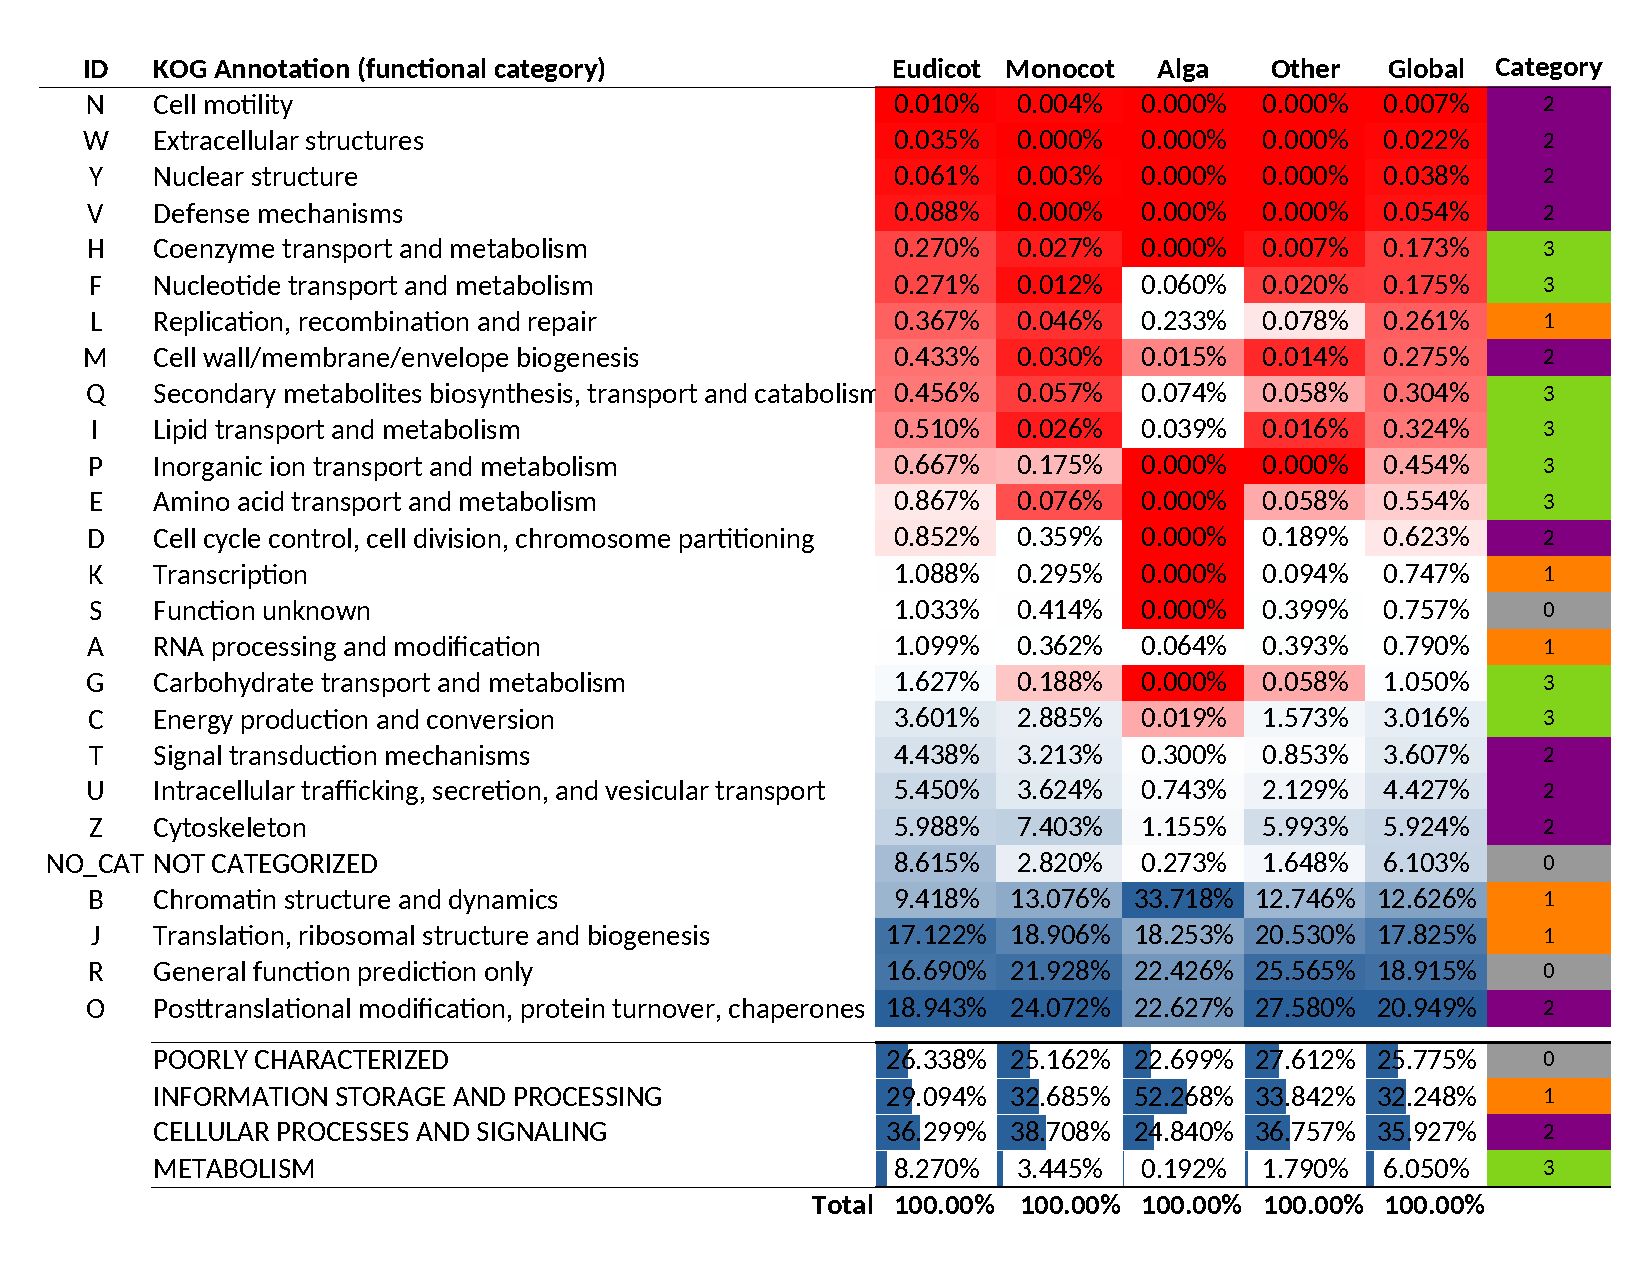
\includegraphics[width=\textwidth]{figures/Heatmap_EMAO}
\caption{Heatmap of the normalized KOG category frequencies 
observed in Phytozome, along with a summary of their 
functional relevance}
\label{fig:EMAO}
\end{figure}


Figure~\ref{fig:EMAO} shows the average of normalized frequency 
for the Phytozome Database. The KOG categories 
appearing the most are ``Posttranslational modification, 
protein turnover, chaperones" (O, 20.95\%), ``General function 
prediction only" (R, 18.91\%), ``Translation, ribosomal 
structure and biogenesis" (J, 17.82\%), and ``Chromatin 
structure and dynamics" (B, 12.62\%). The least frequent 
categories are ``Cell motility" (N, 0.007\%), ``Extracellular 
structures" (W, 0.022\%), and ``Nuclear structure" 
(Y, 0.038\%). The average and median normalized frequency 
for KOG categories are 3.84\% and 0.685\%, respectively. 

% Comparison of KOG category frequencies among different taxonomic groups (e.g., Monocots, Eudicots, Algae, etc.)
As seen in Figure~\ref{fig:EMAO}, the top 4 represented 
categories are still the same as the mentioned for the whole 
database, although the rank changes for Algae: now the most 
represented category is ``Chromatin structure and 
biogenesis". Especially for the Algae and Other groups, there 
is a lack of representation of several KOG categories, 
leading to red gaps in the shown heatmap.
Another interesting KOG category frequency to look at is 
``Carbohydrate transport and metabolism", because it 
allows distinction between Eudicots (1.63\%) and any other 
group (less than 0.2\%).

Note that the proportion of poorly characterized proteins 
is relatively high for the ``Other" group (around 25\%), 
which suggests a lack of established functional 
categorizations across this diverse cluster of species. 
Similarly, ``Information storage and processing" has a 
greater representation in Algae (52.3\%) than any other 
category. This variation implies potential differences 
in nuclear regulatory processes among these plants.

Another important insight is to look at translational 
and posttranslational processes (categories J and O, 
respectively). These two categories add up to more than 
36\% of all biological groups, showing how significant the 
proteome acts toward these housekeeping tasks.


\subsection{Hierarchical Classification}
\label{sec:results.hierarchy}

% Presentation of the hierarchical organization of plant 
% species based on KOG counts

\begin{figure}[htp]
\centering
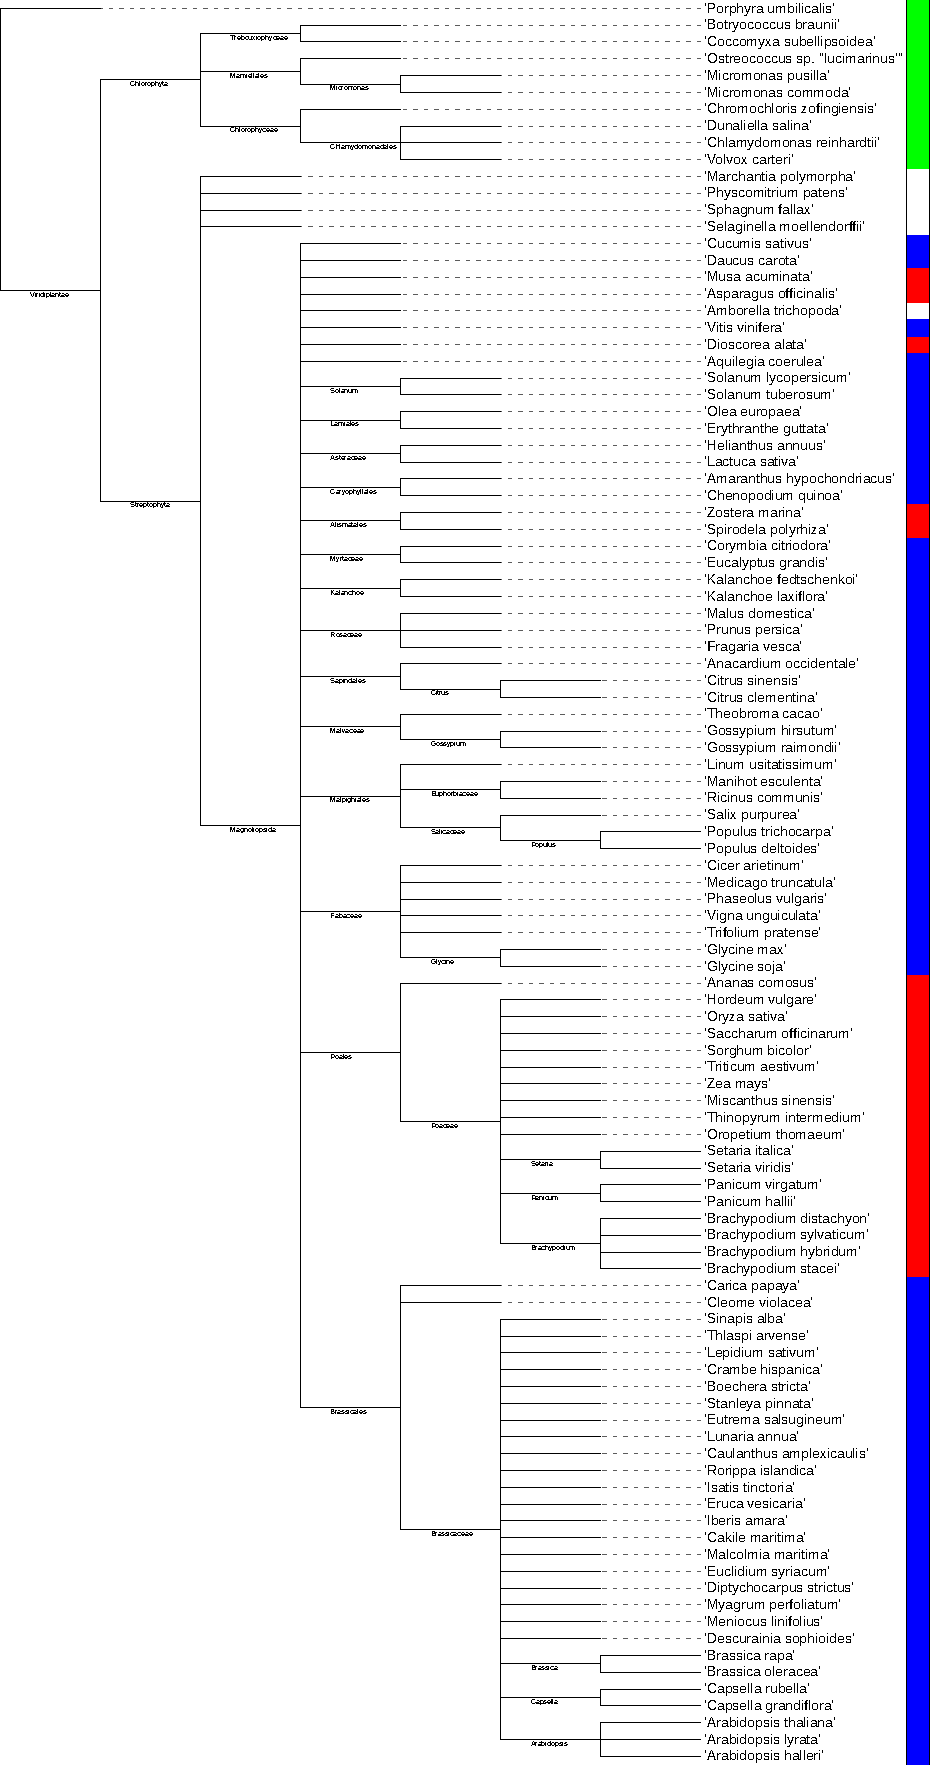
\includegraphics[width=0.9\textwidth]{figures/Taxa}
\caption{Taxonomy tree of the plant species of this study, 
tagged by biological category: Eudicots (blue), Monocots 
(red), Algae (green), and Other (white).
}
\label{fig:taxa}
\end{figure}

Before presenting the results of a hierarchical 
classification based on the KOG category counts, it is 
important to mention that the retrieved dataset consists 
mainly of Eudicotyledons (61.4\%) and Monocotyledons (25.4\%). 
The vast majority of Eudicots belong to the Rosids (56) 
and the Asterids clades (9). Figure~\ref{fig:taxa} presents 
the taxonomic hierarchy of 
the 114 studied plants, using information from the NCBI Taxonomy 
Browser and the online tool Interactive Tree Of Life for 
the tree representation~\citep{letunic2021}. Note that it 
encompasses a wide array of species spanning algae, 
mosses, ferns and flowering plants.

\begin{figure}[htp!]
\centering
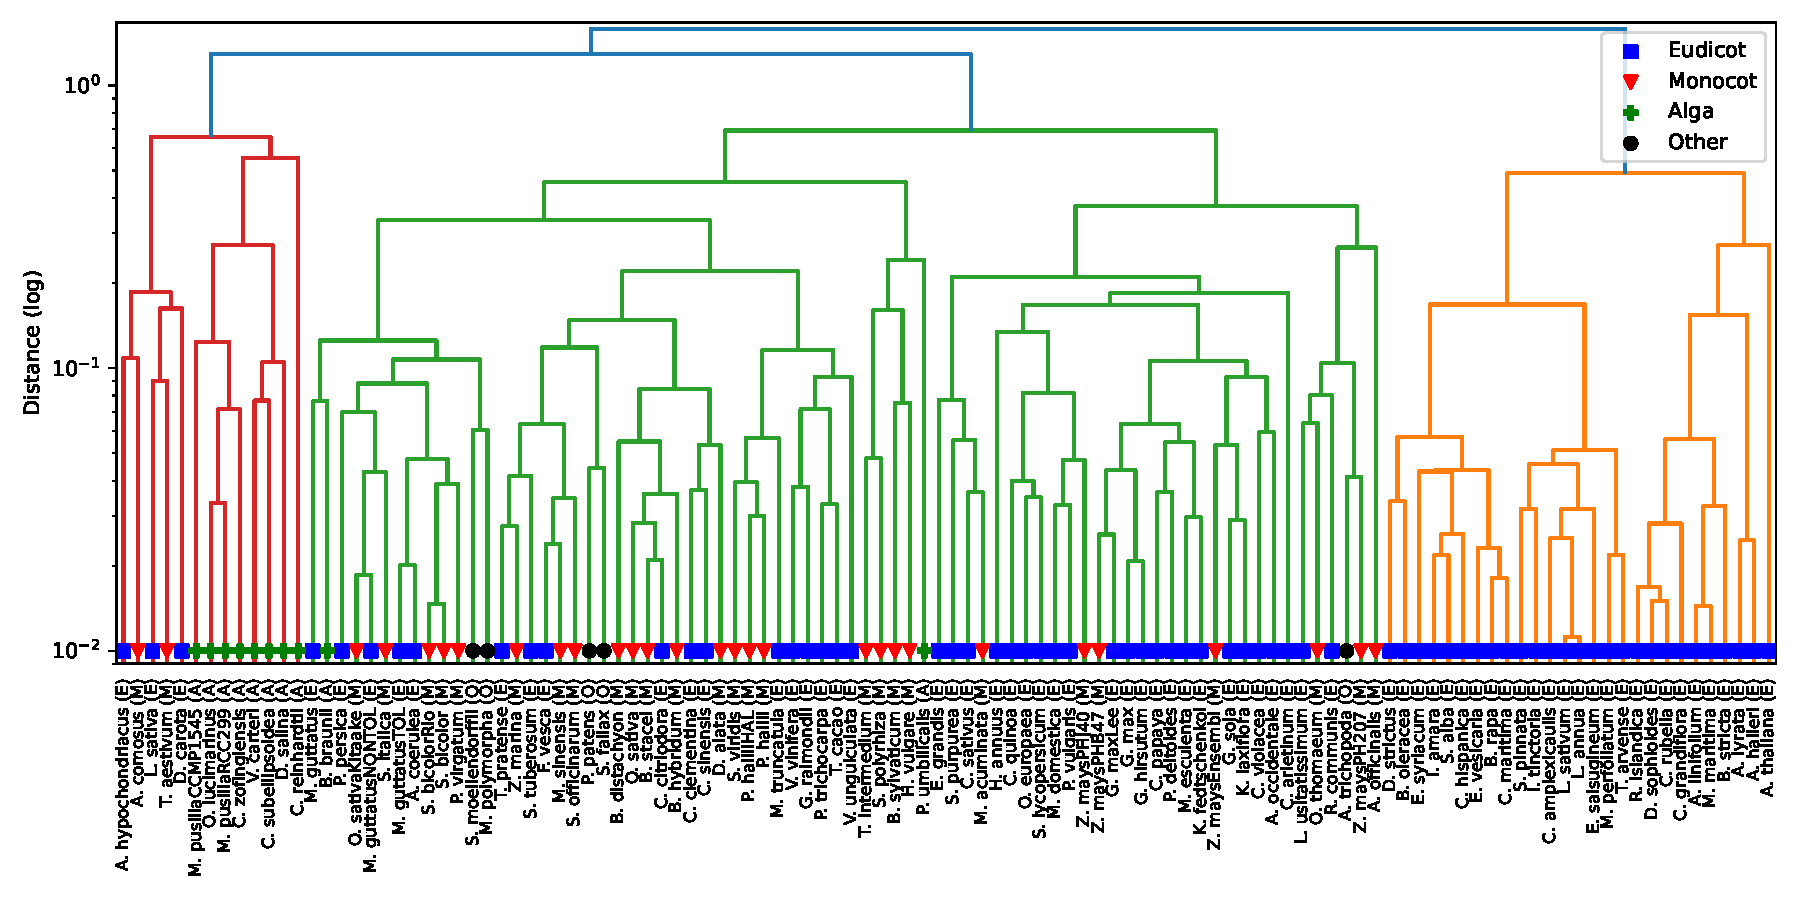
\includegraphics[width=1.05\textwidth]{figures/dendrogram_ward}
\caption{Dendrogram of the Phytozome proteomes, using KOG 
category frequencies as vector representations for 
computing euclidean distance}
\label{fig:dendrogram}
\end{figure}

% Discussion of the clustering patterns and their significance in elucidating plant evolutionary history
% Examination of species groupings and their agreement with known taxonomic classifications
Based on the obtained frequencies of KOG annotations (both 
relative and normalized), the corresponding hierarchical 
classification is carried out, and the resulting 
dendrogram can be observed in Figure~\ref{fig:dendrogram}.
The first aspect that comes unnoticed are the red cluster at 
the left side including many algae and the 
Eudicots-only cluster shown in orange on the right side. 
While the former includes 5 non-algae and leaves out 
two algae, the latter is outstanding on the grounds 
that it perfectly groups all plants from the 
\emph{Brassicaceae} family, a part of the Rosids clade (See 
last 27 rows in Figure~\ref{fig:taxa}).

% Identification of interesting clusters and their potential evolutionary implications
Upon further analysis, it can be seen that the Other KOG 
category splits into \emph{A. Trichopoda}, and two groups 
of two plants each. Apart from those clusters, few relevant 
clusters of different or the same genera appear, beside from 
\emph{Arabidopsis}, \emph{Citrus}, and \emph{Sorghum}, which 
are correctly clustered.

Furthermore, Figure~\ref{fig:clustermap} displays a 
heatmap showing both a hierarchical clustering on the KOG 
categories and on the species, as previously depicted 
in detail. Further analysis of the clustering shows 4 clearly 
differentiated clusters, also related to the ranking shown in 
Figure~\ref{fig:EMAO}:

\begin{figure}[htp]
\centering
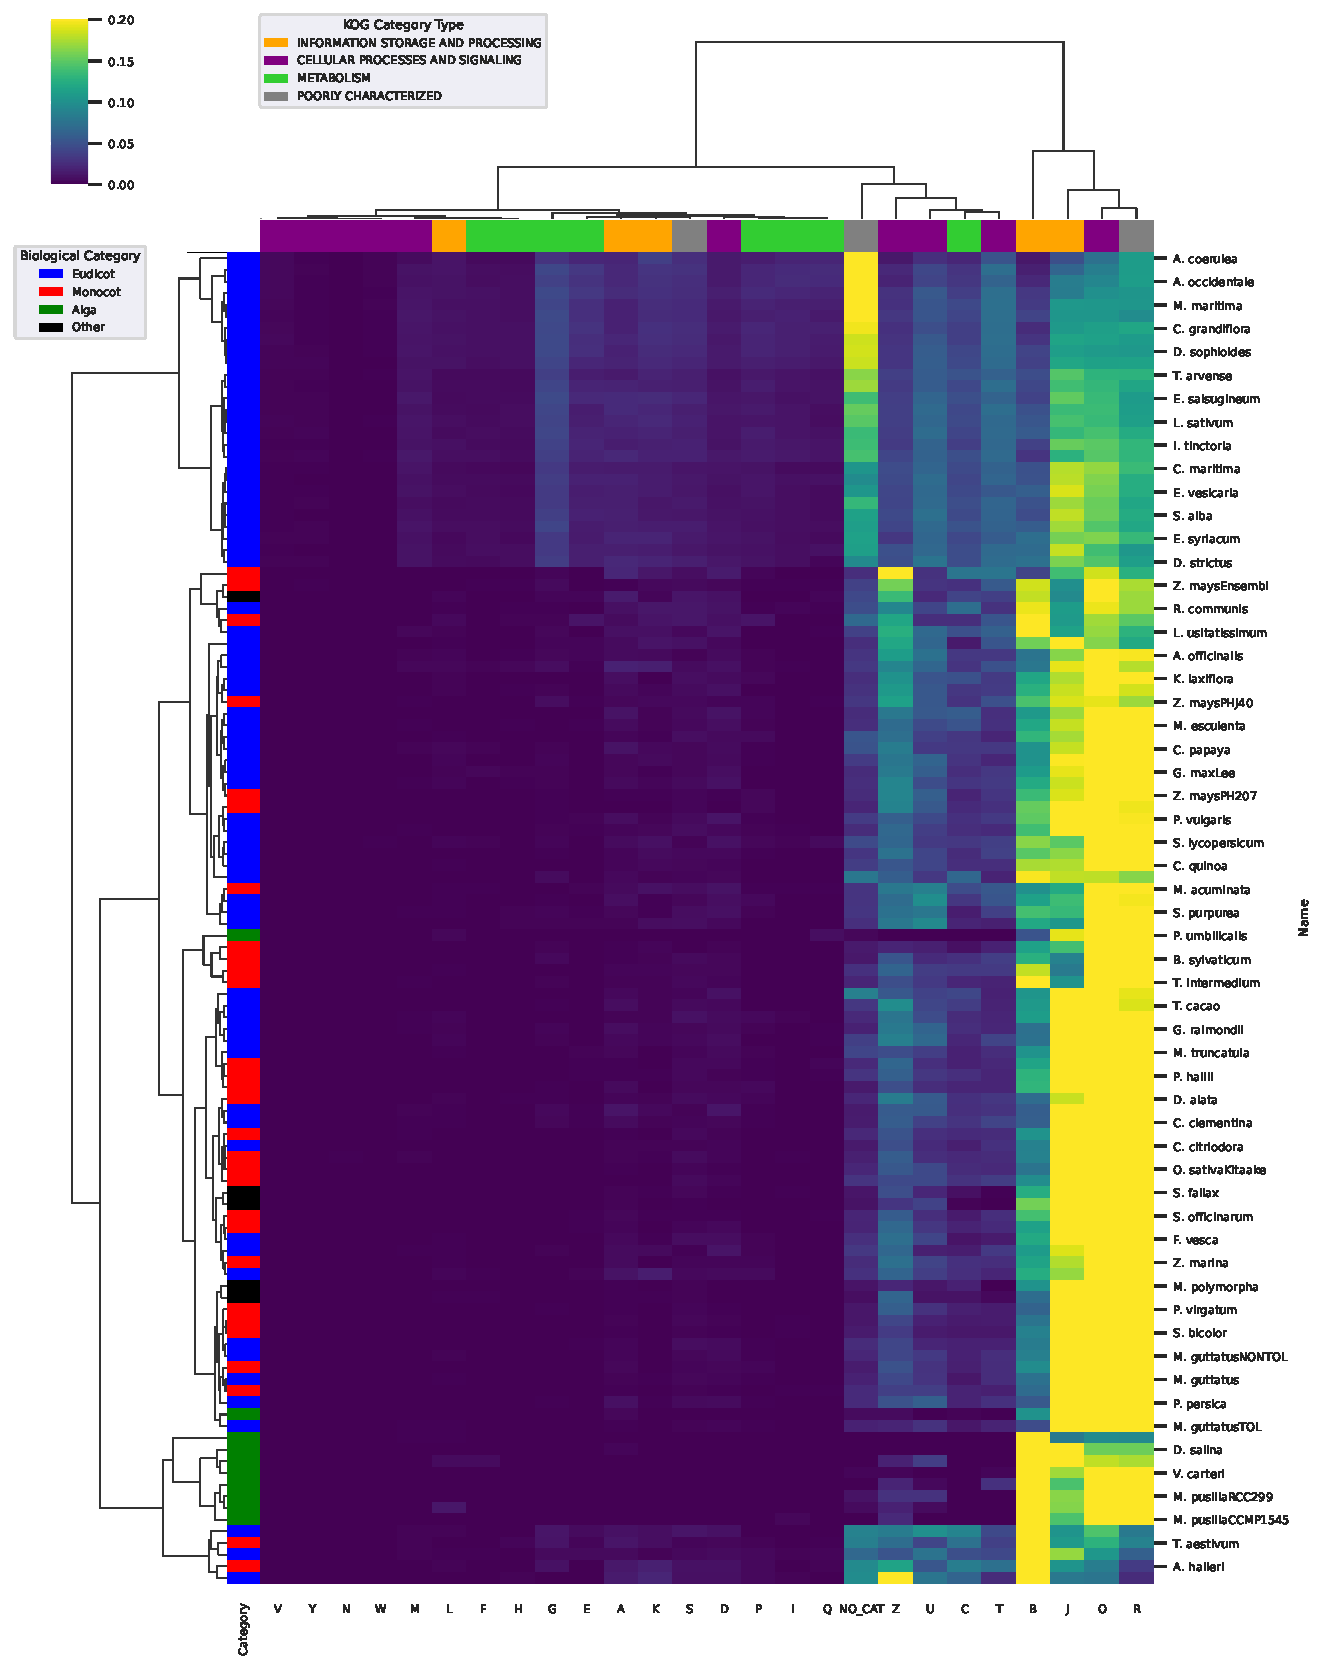
\includegraphics[width=\textwidth]{figures/clustermap}
\caption{Heatmap of the normalized KOG category frequencies 
observed in Phytozome, along with hierarchical clustering 
on categories and on species}
\label{fig:clustermap}
\end{figure}

\begin{enumerate}
\item Categories B, J, O, and R are the most abundant. A 
predominance of processes related to genetic information 
processing and regulation can be observed in this cluster.
\item Categories \verb|NO_CAT|, Z, U, C, and T. This 
cluster revolves 
mostly around cellular dynamics and signaling, although the 
presence of \verb|NO_CAT| suggest a diverse set of functions.
\item Categories G, E, A, K, S, D, P, I, and Q suggest that 
this cluster is associated with diverse metabolic and 
regulatory processes, emphasizing cellular diversity and 
adaptability.
\item Categories V, Y, N, W, M, L, F, and H are related to 
cellular structure, integrity, defense and maintenance.
\end{enumerate}



\subsection{Comparison between Gene Ontology and Phytozome}
\label{sec:results.phytozome-go}

% Summary of the mean and standard deviation of KOG and GO category frequencies
After computing the relative and normalized KOG frequency 
counts for both Phytozome and GO proteomes, the analysis 
results are presented in Figure~\ref{fig:GO}. Note that 
although relative values are not very similar, 
the difference is almost indiscernible between the normalized 
frequency values for both databases. Furthermore, the result 
of using the Spearman's rank correlation coefficient is 0.98, 
suggesting minor differences between the two databases. The 
correlation coefficients shown below correspond to the 
computation against the normalized Phytozome ranking.

\begin{figure}[htp!]
\centering
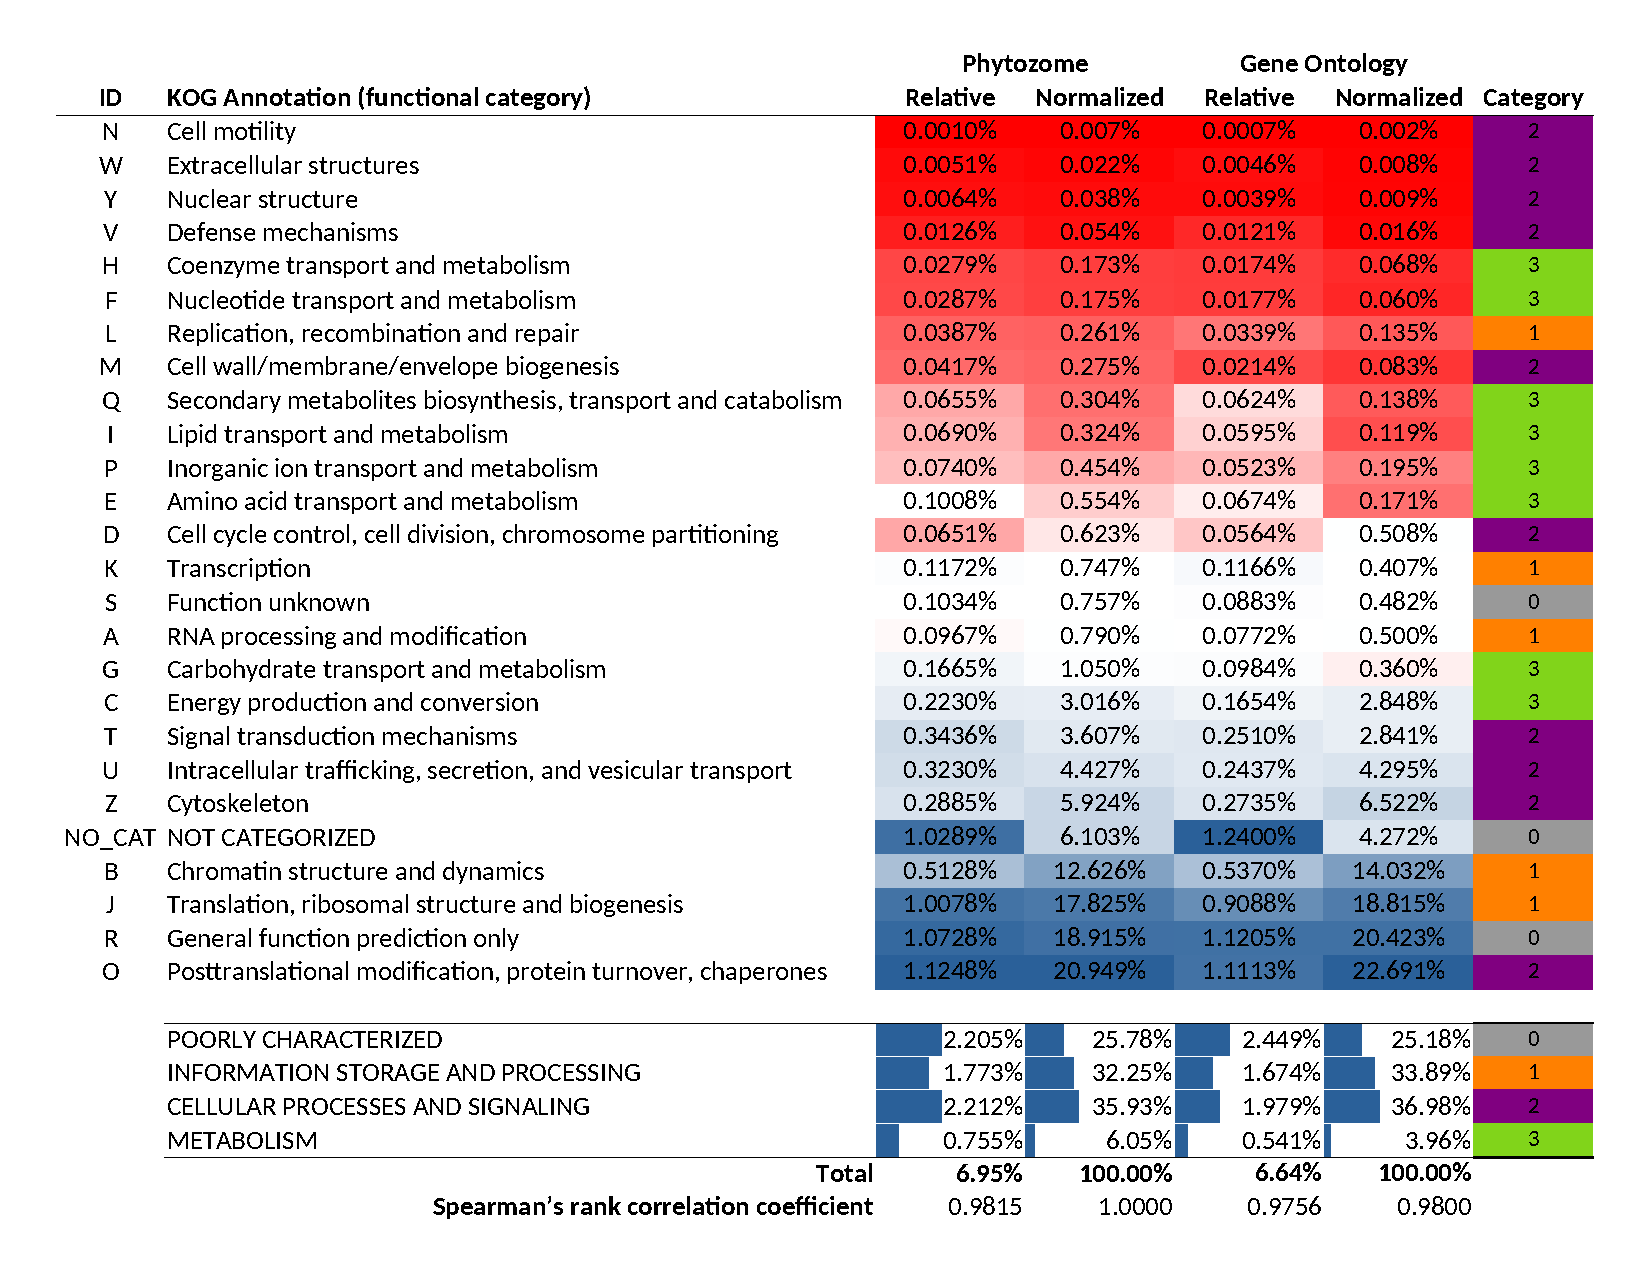
\includegraphics[width=\textwidth]{figures/Heatmap_GO}
\caption{Heatmap of the normalized KOG category frequencies 
observed in Phytozome and GO}
\label{fig:GO}
\end{figure}

Few categories change their relative order in the normalized 
GO ranking, such as ``Cytoskeleton (Z)", ``Carbohydrate 
transport and metabolism (G)", ``Cell cycle control, cell 
division, chromosome partitioning (D)", ``Inorganic ion 
transport and metabolism (P)", and 
``Cell wall/membrane/envelope biogenesis (M)". Besides, 
categories such as ``cell wall/membrane/envelope 
biogenesis (M)" and ``secondary metabolite biosynthesis, 
transport, and catabolism (Q)" show differential 
enrichment in Phytozome compared to Gene Ontology. 
This could indicate variations in the emphasis between 
the two databases.




\section{Discussion and Conclusion}
\label{sec:conclusion}

In this study, a comprehensive exploration of protein 
sequences within the Plantae kingdom is conducted, with 
particular focus on emerging patterns and relationships 
based on KOG category annotations. The results reveal 
insights into the diversity and functional adaptations of 
plant proteomes, shedding light on their adaptive history 
and potential ecological implications. This section 
synthesizes the current findings and provides a broader 
context for their importance.


\subsection{KOG Category Counts Analysis}
\label{sec:conclusion.kogcount}

The analysis of KOG category counts across the 114 plant 
proteomes reveals notable patterns of protein functional 
distribution. Proteomes show varying degrees of 
representation, with \emph{A. thaliana} standing out as 
the best-represented proteome. Other plants, although under 
represented, have an important role in human nutrition or 
health industries. An example is the unicellular green 
alga \emph{D. salina}, whose 
biomass or its extracts have been shown to produce 
positive effects on the treatment of cardiovascular 
diseases and cancer, as well as immunomodulatory and 
anti-inflammatory properties~\citep{hyrslova2022}. 
Carrot (\emph{D. carota}) is another plant 
with a low representation in this study but with an 
outstanding importance due to its antioxidant, 
anti-inflammatory, plasma lipid modification, and 
antitumor properties, which can help reduce the risk of 
cancer and cardiovascular diseases~\citep{ahmad2019}. The 
least represented plant \emph{A. trichopoda} has a rich 
phytochemical landscape that may have potential applications 
in the pharmaceutical and biotechnology industries, due to 
its diverse glycosylated flavonoids, anthocyanins, and 
proanthocyanidins~\citep{wu2019}. 

Considering the normalized count results shown in 
Figure~\ref{fig:EMAO}, there are many aspects to consider.
First, Eudicots and Monocots, the two most closely 
related groups, shows some differences in functional 
categories related to metabolism. Namely, a rupture 
in the trend can be seen on 
the categories of transport and metabolism of inorganic ions 
(P), amino acids (E), and carbohydrates (G). These 
differences could be associated to core differences between 
the two groups at the physiological level, especially 
regarding nutrient acquisition: Eudicots have one main root 
(taproot) where other smaller roots branch off, while 
Monocots have more fibrous roots webbing off in different 
directions~\citep{freschet2021}. Furthermore, evidence 
indicates that metabolic pathways related to nitrogen 
uptake, carbohydrate accumulation, and metal 
transport show differences between Eudicots and 
Monocots~\citep{yang2020,tian2016}.
Secondly, algae display a lack of representation on some 
functional categories, most of them related to cellular 
processes and signaling. On the other hand, the category 
Chromatin structure and dynamics (B) stands out among other 
categories and biological groups. This behavior can also 
be noted on Figure~\ref{fig:clustermap} for the cluster
related to most algae.
In this regard, evidence shows that the genome of \emph{C. 
reinhardtii} has an unusual pattern of methylation when compared 
to other plants or animals~\citep{bacova2020}. Furthermore, 
\cite{vigneau2021} explain that DNA methylation seems to govern 
speciation in plants: in green algae, it occurs in gene-poor 
regions, while in bryophytes marks genes and is crucial for the 
life cycle of the plant. On the other hand, DNA methylation for 
\emph{Arabidopsis} and Angiosperms occurs by silencing some 
gametophyte-specific genes.

Overall, the varying 
representation of KOG categories among different taxonomic 
groups, such as Eudicots, Monocots, and Algae, provides 
insights into potential differences in functional roles 
and adaptations.


\subsection{Hierarchical Classification Results}
\label{sec:conclusion.hierarchy}

The hierarchical organization of plant species based on 
KOG frequency counts highlights clusters that align with 
both known taxonomic classifications and adaptive 
relationships. The presence of distinct clusters, 
particularly the \emph{Brassicaceae} cluster and the 
algae-rich group, reflects the diversity within the 
Plantae kingdom and the similarities on a broad approach to
hierarchical classification in comparison to the taxonomic tree.
Important to note is the fact that the 5 non-algae plants related 
to the latter group have some agricultural importance: Carrot 
(\emph{D. carota}), wheat (\emph{T. aestivum}), lettuce 
(\emph{L. sativa}), pineapple (\emph{A. comosus}), and 
prince's-feather (\emph{A. hypochondriacus}).

The emergence of few well-defined mini-clusters, including 
\emph{A. thaliana}, \emph{Citrus}, and \emph{Sorghum}, 
calls attention to the shared functional roles among 
species from the same genus. The placement of 
\emph{A. trichopoda} and the plants from the Monocot and 
Other biological groups is a matter worth a closer look, 
since no conclusion about their classification can be 
established based on these results.

Similar approaches can be found in the literature. For 
instance, The \emph{GeneFamilyPhylogenyBuilder} tool from 
PlantTribes2 computes a hierarchical classification of 
plants based on multiple sequence 
alignment~\citep{wafula2023}. In turn, PlantTribes2 uses 
RAxML or FastTree 
algorithms for estimating maximum likelihood (ML) 
phylogenetic trees. This is different to our approach 
because functional categories are not considered in the 
hierarchical classification.

Another approach can be found in The Plant Orthology Browser, 
which uses gene models for 20 fully sequenced plant genomes 
and leverages GO annotations to determine sets of conserved 
synteny blocks~\citep{tulpan2017}. This resource, as well as
InParanoiDB 9~\citep{persson2023}, are focused on ortholog 
prediction and use functional annotations for finding such 
ortholog groups. However, our goal is to assess the 
importance of those annotations on adaptive processes.


\subsection{Comparison between Gene Ontology and Phytozome}
\label{sec:conclusion.comparison}

The comparison between Phytozome-based and GO-based 
classifications revealed a high degree of concordance, 
with a Spearman's rank correlation coefficient of 0.98. 
This confirms the robustness of the KOG annotations and 
their alignment with GO annotations in characterizing 
protein functions~\citep{tatusov2003}. 
The minor differences observed in the 
rankings of certain categories stress the complementary 
nature of these databases in providing a comprehensive 
understanding of protein functionality. Differential 
enrichment of certain categories between the databases 
hints at distinct emphasis in annotation curation.

Regarding the inference of species relationships, the 
approach presented in this study also differs from the one 
presented by~\cite{wafula2023} in PlantTribes2, where 
functional annotations are extracted from Gene Ontology, 
InterPro/Pfam protein domains, The Arabidopsis Information 
Resource (TAIR), UniProtKB/TrEMBL, and UniProtKB/Swiss-Prot.
However, the approach presented in this study differs from 
those of PlantTribes2, The Plant Orthology Browser, and 
InparanoiDB because it uses the counting of annotated proteins 
for each functional category in KOG, instead of directly using 
some form of sequence alignment. It does not mean that the 
presented approach uses no alignment whatsoever, but it is only 
a preprocessing that helps in retrieving the mentioned counts.



\subsection{Conclusion}
\label{sec:conclusion.conclusion}

The comprehensive analysis of protein 
sequences within the Plantae kingdom using KOGs has 
unveiled intricate patterns of functional distribution, 
evolutionary relationships, and shared annotations with 
the GO database. Namely, This study presents 
how the functional annotations vary among the defined plant 
clusters. These averaged distributions of category counts 
can be used as an initial criterion for classifying a 
unobserved organism based on how similar its own category counts 
are from each cluster. Furthermore, the applied methodology 
for identifying these functional annotation distributions 
can be extended to more organisms or even applied again 
from scratch for other life kingdoms, where a 
functional criterion for classification could elucidate 
additional relationships between organisms. A broad coverage of 
the studied kingdom is highly encouraged.

Furthermore, some clusters found by the methodology presented 
in this study are similar to phylogenetic groups, such 
as the \emph{Brassicaceae} or the algae-rich cluster, as observed
in Figure~\href{fig:clustermap}. This, in 
turn, shows that adaptive processes could be closely related 
to how the proteome responds to environmental cues, although 
the direction of causality and if such causality between the 
two even exists, is not assessed in this study.
Overall, the integration of bioinformatics tools, 
hierarchical classification, and statistical analyses provides 
a deeper understanding of plant biology and adaptive processes. 
This study paves the way for further research and 
applications in molecular biology, bioinformatics, and 
proteomics, ultimately enhancing our knowledge of 
plant-environment interactions and adaptive responses to 
changing conditions.







\backmatter

\vspace{1in}

\textbf{Author contribution statement} Conceptualization: N.L.-R. and 
F.T.-T.; Methodology: N.L.-R. and F.T.-T.; Software: N.L.-R.; 
Validation: N.L.-R.; Investigation: N.L.-R.; 
Data curation: N.L.-R.; 
Writing---original draft preparation: N.L.-R.; 
Writing---review and editing: F.T.-T., J.F. and C.R.; 
Project administration: J.F and C.R.; 
Funding acquisition: J.F. and C.R.;
All authors have read and agreed to the published version of the 
manuscript.

\textbf{Acknowledgments}
We would like to thank prof. Oliver Ebenhöh, Camila Riccio and 
Mauricio Ramírez-Castrillón for their helpful comments and 
insights.

\textbf{Funding}
This work was partially funded by the ``OMICAS program:
Optimización Multiescala In-silico de Cultivos Agrícolas 
Sostenibles (Infraestructura y validación en Arroz y Caña de 
Azúcar)'' Scientific Ecosystem belonging to the Colombia 
Científica Program, sponsored by The World Bank, The 
Ministry of Science, Technology and Innovation (MINCIENCIAS), 
ICETEX, the Colombian Ministry of Education and the Colombian 
Ministry of Commerce, Industry and Tourism, under GRANT ID: 
FP44842-217-2018, OMICAS Award ID: 792-61187.

\textbf{Data availability}
The datasets used and/or analyzed during 
the current study are available from the corresponding author on 
reasonable request.


\section*{Declarations}

\textbf{Conflicts of interest}
The authors declare no conflicts of interest relevant to the content 
of this manuscript.

\textbf{Ethics approval and consent to participate}
Not applicable.

\textbf{Consent for publication}
Not applicable.

\textbf{Open Access}
This article is licensed under a Creative Commons 
Attribution 4.0 International License, which permits use, sharing, 
adaptation, distribution and reproduction in any medium or format, as long
as you give appropriate credit to the original author(s) and the source,
provide a link to the Creative Commons license, and indicate if changes
were made. The images or other third party material in this article are
included in the article's Creative Commons license, unless indicated
otherwise in a credit line to the material. If material is not included 
in the article's Creative Commons license and your intended use is not
permitted by statutory regulation or exceeds the permitted use, you will
need to obtain permission directly from the copyright holder. To view a
copy of this license, visit \url{http://creativecommons.org/licenses/by/4.0/}

%%===========================================================================================%%
%% If you are submitting to one of the Nature Portfolio journals, using the eJP submission   %%
%% system, please include the references within the manuscript file itself. You may do this  %%
%% by copying the reference list from your .bbl file, paste it into the main manuscript .tex %%
%% file, and delete the associated \verb+\bibliography+ commands.                            %%
%%===========================================================================================%%

\bibliography{refs}
%% if required, the content of .bbl file can be included here once bbl is generated
%%\input sn-article.bbl


\end{document}
